\documentclass[a4paper]{article}
\usepackage[hidelinks]{hyperref}
\usepackage[parfill]{parskip}
\usepackage[%
  left=3cm,
  right=3cm,
  top=1.5cm,
  bottom=2cm,
  marginparwidth=0cm,
  marginparsep=0mm
]{geometry}
\usepackage{booktabs}
\usepackage{tabularx}
\usepackage[noabbrev,nameinlink]{cleveref}
\usepackage{graphicx}
\usepackage{float}
\usepackage{xcolor}

\graphicspath{{./images/}}

\title{AI and Games Semester 2 Project Report}
\author{\textbf{Group 16} \\ Evripidis Christodoulides, Jonathan Haylett, Wenchang Liu,
Huan Yang}
\date{\today}

\begin{document}
\maketitle
\tableofcontents

\pagebreak
\section{Task Overview}
The objective of this project is to develop a leader AI program that tries to
get as much profit as it can by publishing its price every day for 30 days of
simulation in a Stackelberg game against 3 follower AI programs respectively.
The process of achieving this objective is divided into 2 main steps: estimating
the reaction function of the follower, and calculating the price to publish.

As mentioned in \cref{sub:calculating_price}, since the procedure after
estimating the reaction function of the follower is the same, we will mainly
discuss how to do the regression to estimate the reaction function more
accurately.
We have implemented a linear regression leader agent with an online learning
algorithm that can make a greater profit than SimpleLeader.
Also, we experimented with other regression models including decision trees,
SVM, etc.
Eventually, we propose some other ideas which may perform better for this
task, but we did not have time to implement them.


\subsection{Estimating the Reaction Function of the Follower}
In order to determine the price we publish for each day, the leader will try to
estimate the reaction of the follower to the price it publishes, i.e.\
$U_F=F(U_L)$.
Theoretically, the more accurate our estimation is, the more profit we will get.
The data that we have available to do the estimation with is the 100 pairs of
historical data.
This is a regression task where we need a mapping function that maps a price
that the leader publishes to a price that the follower publishes.
The idea is that if we can train the model to fit most of the historical data,
it can make predictions that are close to what the follower will actually
publish.
Such models including linear regression and its variations.

\subsection{Calculating the Price to Publish}%
\label{sub:calculating_price}

After estimating the reaction function of the follower, we can then bring the
reaction function into the demand model of the leader, and then we will receive
a formula with only one parameter --- $U_L$.
In order to calculate the maximum value of this formula, we will have to
differentiate it to find which $U_L$ can make it reach the maximum value, and
this $U_L$ is what we will publish.
Finally, we can calculate the daily profit.
No matter what models we use for learning the reaction function, the process for
calculating the price to publish is always the same.

\section{Linear Regression with Online Learning}%
\label{sec:linearonlinelearning}
\subsection{Linear Regression}
The simplest regression idea is to use linear regression.
The basic idea of it is that we assume the follower's reaction function is a
% TODO: Is "i.e. say" really the best way to put it?
linear function, i.e.\ say $U_F = a \cdot U_L + b$, where $a$ and $b$ are unknown
parameters, and an approximation function $U_F = a^* \cdot U_L+ b^*$, where $a^*$
and $b^*$ are the parameters we need to calculate.
Then we use the square error sum at the given data to measure the closeness,
and we update the parameters $a^*$ and $b^*$ using the historical data we have
so that our predicted linear function $U_F = a^* \cdot U_L+ b^*$ can be as close
to the original linear function as possible.

\subsection{Online Learning: The Moving Window Approach}
In addition to the 100 days of historical data, we still have new data generated
during the simulation.
The moving window approach is designed to make use of these pieces of
information.
For example, if we use the window size 100, then for each new day of the
simulation, we will calculate the parameters using the previous 100 days' data
starting from the current day.
In other words, we will discard data that has reached a certain age and take an
equal amount of new data into consideration.
The advantage is that if the environment is continuously changing, we can
discard outdated data and update our model with the latest data.

\subsection{Algorithm Implementation}
\begin{figure}[H]
  \centering
  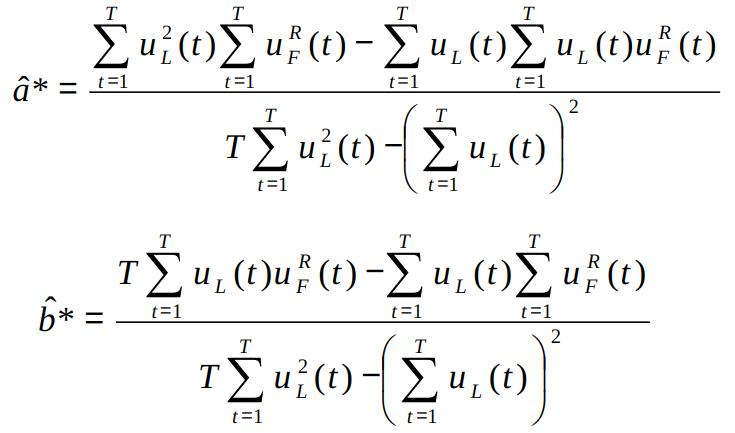
\includegraphics[width=6cm]{linear-formula}
  \caption{Formulae for calculating $a^*$ and $b^*$}%
  \label{fig:linear-formula}
\end{figure}

For each new day, we will first calculate the parameters $a^*$ and $b^*$
according to the formulas in \cref{fig:linear-formula} using the same amount of
data as the window size, then we put $U_F = a^* \cdot U_L + b^*$ into the daily
profit formula $(U_L - 1) \cdot (2 - U_L + 0.3 \cdot U_F)$ and get
$(U_L - 1) \cdot (2 - U_L + 0.3 \cdot (a^* \cdot U_L + b^*))$,
i.e. $(U_L - 1) \cdot (2 - U_L + 0.3 \cdot a^* \cdot U_L + 0.3 \cdot b^*)$.
We then differentiate this formula to get
$U_L \cdot (-2 + 0.6 \cdot b^*) + 3 + 0.3 \cdot a^* - 0.3 \cdot 0b^*$, and let
the differentiated formula equals 0, then we can solve the equation to get
$U_L = (-3 - 0.3 \cdot a^* + 0.3 \cdot b^*) / (-2 + 0.6 \cdot b^*)$ which will
theoretically make the leader receive maximum profits.
Eventually, we just put the calculated $a^*$ and $b^*$ into this formula to get
the price we should publish.
The flow diagram of the linear regression algorithm with the moving window
approach is shown below in \cref{fig:moving-window}.

\begin{figure}[H]
  \centering
  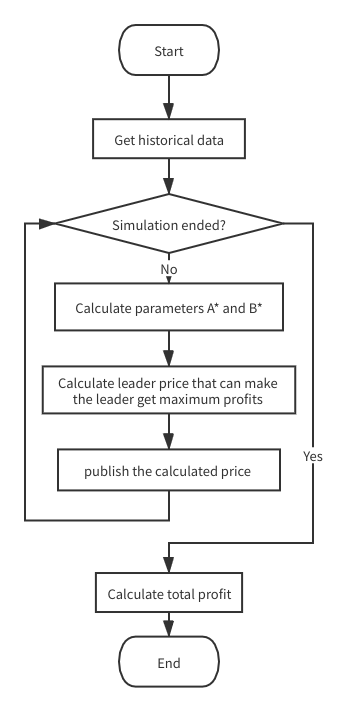
\includegraphics[width=7cm]{moving-window}
  \caption{Flow Diagram of Linear Regression with Moving Window Algorithm}%
  \label{fig:moving-window}
\end{figure}

\subsection{Evaluation Based on Profits (Moving Windows)}
We tested our model with different window sizes against all followers, and we
also compared our profits to the given SimpleLeader's profits.
The results are shown below in \cref{table:moving_window_eval}.

\begin{table}[H]
  \centering
  \begin{tabularx}{\textwidth}{X X X X}
  \toprule
  \textbf{Leader} & \textbf{Mk1} & \textbf{Mk2} & \textbf{Mk3} \\
  \midrule
  \textcolor{blue}{SimpleLeader} & \textcolor{blue}{17.491040}
                                 & \textcolor{blue}{16.897467}
                                 & \textcolor{blue}{19.423810} \\
  \midrule
  Window Size 10 & 17.405104 & 16.932770 & 19.411194 \\
  \midrule
  Window Size 25 & 17.484606 & 16.953413 & 19.464302 \\
  \midrule
  Window Size 40 & 17.535341 & 16.95259 & 19.488014 \\
  \midrule
  Window Size 55 & 17.547180 & 16.952982 & 19.487911 \\
  \midrule
  Window Size 70 & 17.552155 & 16.953724 & 19.488184 \\
  \midrule
  \textcolor{red}{Window Size 85} & 17.554714 & 16.953964
                                  & \textcolor{red}{19.488335} \\
  \midrule
  Window Size 100 & 17.555769 & 16.955841 & 19.488330 \\
  \midrule
  Window Size 115 & 17.556887 & 16.956198 & 19.488293 \\
  \midrule
  \textcolor{red}{Window Size 130} & \textcolor{red}{17.557184}
                                   & \textcolor{red}{16.956450} & 19.488283 \\
  \bottomrule
\end{tabularx}

  \caption{Comparison of Profits with Different Window Sizes}%
  \label{table:moving_window_eval}
\end{table}

As we can see from the table, we made more profits by estimating the follower
reaction function and publishing our price according to the reaction function
than randomly publishing prices like the SimpleLeader.
The best performance against Mk1 and Mk2 is achieved by using window size 130,
and the best performance against Mk3 is achieved using window size 85.

\section{Evaluation of Different Regression Models}
Apart from implementing the linear regression in Java, we explored more
regression models and evaluated them with R-squared scores with Scikit-learn.
The R-squared score is a good way to evaluate the performance of a regression.
The score of a regression can be ranged from 0 to 1, which is a relative
evaluation.
Such a score has an advantage over other absolute scores in that we cannot
easily determine how high an absolute score can be regarded as a good score.
However, it is safe to say an R-squared score close to 1 is a good one.

\subsection{Evaluation of Linear Regression}
We evaluated linear regression on mk1, mk2, mk3 historical data, and their
R-squared scores are 0.19, 0.11, 0.72 respectively.
As we know, an R-squared score below 0.4 means the regression is not that good,
so our linear regressions are not good enough except for mk3.

\begin{figure}[H]
  \centering
  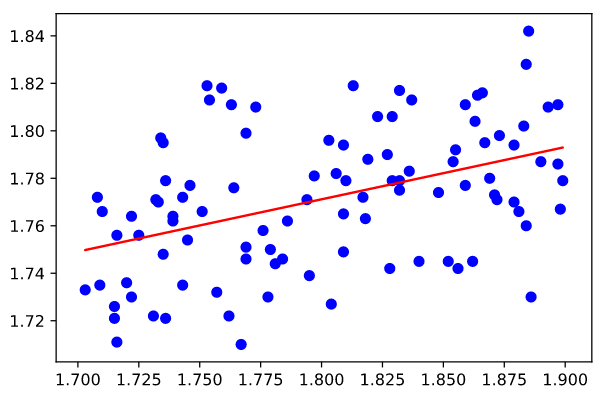
\includegraphics[width=10cm]{linear-mk1}
  \caption{Linear Regression on Mk1 Historical Data}%
  \label{fig:linear-mk1}
\end{figure}

In linear regression, we can imagine that we need to draw a straight line to fit
most of the data points and make sure other data points are not too far away.
But as we can see in \cref{fig:linear-mk1}, the data points from mk1 are
scattered, so it is very hard to fit many points with a single line.
This is why we want to experiment with other non-linear regression models and
see if they can achieve better R-squared scores.

\subsection{Evaluation of Decision Tree Regression}
The decision tree regression can learn complex rule-based patterns; however, it
seems to suffer from overfitting issues here according to our experiments.
We split the historical data into a training set and testing set.
While the decision tree regression model achieves a 0.93 R-squared score on the
training set, it achieves a score of -1.58 on the testing set.
% Bit unsure about whethere I edited this paragraph in a way that is accurate.
A negative value means the model can be arbitrarily worse.
As shown in \cref{fig:decisiontree-mk1}, the model seems to find the wrong way
to fit the data points.

\begin{figure}[H]
  \centering
  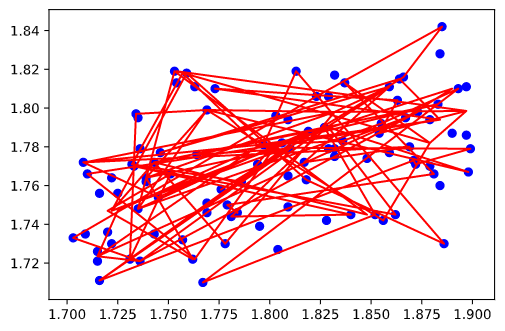
\includegraphics[width=10cm]{decisiontree-mk1}
  \caption{Decision Tree Regression on Mk1 Historical Data}%
  \label{fig:decisiontree-mk1}
\end{figure}

\subsection{Other Regression Experiments}
We have also tried other popular regression models including SVM, KNN, random
forest, and AdaBoost on Mk1 and none of them worked better than linear
regression.
\Cref{table:regression_experiments} shows the R-squared scores obtained from
these experiments.

\begin{table}[H]
  \centering
  \begin{tabularx}{\textwidth}{X X X}
  \toprule
  \textbf{Model} & \textbf{Training R Score} & \textbf{Testing R Score} \\
  \midrule
  Linear & 0.20563019704498864 & 0.12381456611660624 \\
  \midrule
  Decision Tree & 0.9334617516195677 & -1.5818682765183536 \\
  \midrule
  SVM & -0.003296979174702175 & -0.17390958609995066 \\
  \midrule
  KNN & 0.3395643813770154 & 0.06677303550060165 \\
  \midrule
  Random Forest & 0.7072866944733289 & -0.047113503710458415 \\
  \midrule
  AdaBoost  &0.40155919508932547 & 0.05755037520545825 \\
  \bottomrule
\end{tabularx}

  \caption{Results of Experimentation with Different Regression Models on Mk1
  Historical Data}%
  \label{table:regression_experiments}
\end{table}

\section{Other Ideas -- Explore Time Series}
From the results of our experiments, we think it is unlikely that we will be
able to make precise predictions by simply fitting all the historical points
together.
% Maybe this can be made more fluid
The reaction function might be affected by the time series.
One possibility is that there are several sets of parameters for a follower
based on the current date.
Another possibility is that the follower is not only reacting to the leader 
simply according to the current published price of the leader, but also taking
several previous days' data into consideration.
We have thought about several approaches to explore the time series problem.

\subsection{Calculate slope between current day and previous day}
Assuming the follower has several different linear reaction functions, then each
function will have a different slope.
Therefore, theoretically, after we calculate the slope between the current day's
price and the previous day's price
$\frac{(follower\_i - follower\_i-1)}{(leader\_i - leader\_i-1)}$ as y-axis and
using dates as x-axis to plot the line graph, we may see the turning point of
the slopes and that is when the parameters have changed.
If we can chunk all the historical data into several parts, then we can do the
same as \cref{sec:linearonlinelearning} to do a more accurate linear regression
for each part separately.

\subsection{Sequential Model}
If the follower decides its price by a sequence of data, e.g.\ previous 3 days'
prices, then a sequential model might help.
If we put all historical data together, it is like the bag of words model in
NLP, which does not consider the sequences of data.
Similarly, we can simulate the skip-gram idea by taking the leader's price from
consecutive several days as the input to the regression model, and do a
multivariable regression.
Alternatively, we can directly try other sequential models such as RNN networks
to predict a sequence of data.

\end{document}
